\documentclass{article}
\usepackage[utf8]{inputenc}
\usepackage{geometry}
\usepackage{hyperref}
\usepackage{multicol}
\usepackage{graphicx}
\usepackage{float}

\geometry{a4paper, total={170mm,257mm}, left=20mm, top=20mm}
\usepackage{graphicx}
\usepackage{titling}

\title{Group A3D: SPARQL Queries and Analytics}
\author{Group A3D}
\date{10th January 2025}

 \usepackage{fancyhdr}
\fancypagestyle{plain}{%  the preset of fancyhdr
    \fancyhf{} % clear all header and footer fields
    % \fancyfoot[R]{\includegraphics[width=2cm]{KULEUVEN_GENT_RGB_LOGO.png}}
    \fancyhead[]{\thedate}
    \fancyhead[L]{SPARQL Queries and Analytics}
    \fancyhead[R]{\theauthor}
}
\makeatletter
\def\@maketitle{%
  \newpage
  \null
  \vskip 1em%
  \begin{center}%
  \let \footnote \thanks
    {\LARGE \@title \par}%
    \vskip 1em%
    %{\large \@date}%
  \end{center}%
  \par
  \vskip 1em}
\makeatother

\usepackage{lipsum}
\usepackage{cmbright}

\usepackage{xcolor}
\usepackage{listings}
\lstdefinelanguage{SPARQL}{
    keywords={SELECT, WHERE, AS, FILTER, OPTIONAL, GRAPH, UNION, PREFIX, ORDER, BY, ASC, DESC, LIMIT, OFFSET, BIND, GROUP, HAVING, COUNT, DISTINCT, SUM, AVG, MIN, MAX, GROUP_CONCAT, SEPARATOR, YEAR, ROUND},
    keywordstyle=\color{blue}\bfseries,
    ndkeywords={a, rdf:type},
    ndkeywordstyle=\color{teal}\bfseries,
    identifierstyle=\color{black},
    stringstyle=\color{red}\ttfamily,
    commentstyle=\color{gray}\itshape,
    sensitive=true,
    morecomment=[l][\color{gray}]{\#}
}
\lstset{
    language=SPARQL,
    basicstyle=\ttfamily\small,
    numbers=left,
    numberstyle=\tiny\color{gray},
    stepnumber=1,
    frame=single,
    breaklines=true,
    captionpos=b,
    tabsize=2,
    showstringspaces=false
}

\begin{document}

\maketitle

\begin{tabular}{@{}ll}
	\textbf{Group members:}
	 & \href{mailto:andrea.bruttomesso.1@studenti.unipd.it}{Andrea Bruttomesso} 2120933 \\
	 & \href{mailto:alessandro.corro.1@studenti.unipd.it}{Alessandro Corr\`o} 2125034   \\
	 & \href{mailto:davide.seghetto@studenti.unipd.it}{Davide Seghetto} 2122548         \\
	 & \href{mailto:andrea.stocco.8@studenti.unipd.it}{Andrea Stocco} 2108885           \\
\end{tabular}

\section{Relationship between Nobel Prize winning ideas and published studies}
\label{sec:nobelTopics}
\begin{lstlisting}
PREFIX spif: <http://spinrdf.org/spif#>
PREFIX : <http://www.semanticweb.org/a3d/ontologies/2024/10/nobelOntology/>
PREFIX xsd: <http://www.w3.org/2001/XMLSchema#>

SELECT ?nobelTopic ?nobel (COUNT(?paper) AS ?numPapers) WHERE {
    {
        SELECT ?paperTopic ?paper WHERE {
            ?paper :hasAbstractTopics ?topics ;
               	:hasYear ?year .
            FILTER (?year = "2004"^^xsd:gYear)
            ?paperTopic spif:split(?topics ",")
        }
    }
    {
        SELECT ?nobelTopic ?nobel WHERE {
            ?nobel :hasMotivationTopics ?topics ;
                :hasYear ?year .
            FILTER (?year = "2004"^^xsd:gYear)
            ?nobelTopic spif:split(?topics ",")
        }
    }
    FILTER (?nobelTopic = ?paperTopic)
}
GROUP BY ?nobelTopic ?nobel
ORDER BY DESC (?numPapers)
\end{lstlisting}

\vspace{1em}

This query shows the topics present in both Nobel Prize motivations and paper abstracts.
For a given year, it returns the number of papers in which a Nobel topic appears.
This query can be used to find correlations between Nobel Prize topics and research
papers.\\
Table \ref{tab:papersNobelTopicsYear} shows the output of this query in 2004.

\begin{table}[H]
	\centering
	\caption{Number of papers per Nobel topic in 2004}
	\begin{tabular}{|l|l|c|}
		\hline
		\textbf{Nobel topic} & \textbf{Nobel Prize} & \textbf{Number of papers} \\ \hline
		protein              & Chemistry 2004       & 28                        \\ \hline
		development          & Peace 2004           & 13                        \\ \hline
		flow                 & Literature 2004      & 8                         \\ \hline
		interaction          & Physics 2004         & 4                         \\ \hline
		discovery            & Chemistry 2004       & 3                         \\ \hline
		discovery            & Physics 2004         & 3                         \\ \hline
		degradation          & Chemistry 2004       & 3                         \\ \hline
		asymptotic           & Physics 2004         & 2                         \\ \hline
		forces               & Economics 2004       & 1                         \\ \hline
		cycles               & Economics 2004       & 1                         \\ \hline
		olfactory            & Medicine 2004        & 1                         \\ \hline
		organization         & Medicine 2004        & 1                         \\ \hline
	\end{tabular}
	\label{tab:papersNobelTopicsYear}
\end{table}

\newpage

Considering the limited number of papers available, the topic ``protein'' appeared
in 28 papers. The high number of papers mentioning this Nobel topic suggests that
it was widely discussed or relevant in 2004.\\
We cannot conclude whether the molecular biology research area was particularly active
in that year, but in Section \ref{moreActiveResearchAreas} we will further
investigate this.\\
Unfortunately, this query is not always useful. In some cases, the
main topics may include words like ``method'' and ``analysis'', which are not
informative enough to determine how extensively a specific topic was studied
in a given year.\\
Due to the distribution of research papers in our dataset across different years,
this query provides more meaningful results for years after 2000.

\newpage

\section{Most active research areas in a year} \label{moreActiveResearchAreas}
\begin{lstlisting}
PREFIX : <http://www.semanticweb.org/a3d/ontologies/2024/10/nobelOntology/>
PREFIX xsd: <http://www.w3.org/2001/XMLSchema#>
PREFIX skos: <http://www.w3.org/2004/02/skos/core#>

SELECT ?category (COUNT(?paper) AS ?numPapers) WHERE {
    ?paper :publishedIn ?venue ;
        :hasYear ?year .
    ?venue :hasJournalCategory ?category .
    ?category skos:broaderTransitive ?sub .
    FILTER (?year = "2004"^^xsd:gYear)
}
GROUP BY ?category
ORDER BY DESC (?numPapers)
\end{lstlisting}

\vspace{1em}

This query shows the number of papers published for each journal subcategory for a given year.
It can be used to identify which research areas were particularly active in that year.\\
Table \ref{tab:papersPerSubcategoryPerYear} continues the analysis started in Section \ref{sec:nobelTopics}.

\begin{table}[H]
	\centering
	\begin{tabular}{|l|c|}
		\hline
		\textbf{Journal Subcategory}            & \textbf{Number of papers} \\ \hline
		Biochemistry Genetics Molecular Biology & 418                       \\ \hline
		Social Sciences                         & 344                       \\ \hline
		Decision Sciences                       & 125                       \\ \hline
		Arts Humanities                         & 74                        \\ \hline
		Business Management Accounting          & 68                        \\ \hline
		Physics Astronomy                       & 65                        \\ \hline
		Neuroscience                            & 55                        \\ \hline
		Health Professions                      & 34                        \\ \hline
		Psychology                              & 27                        \\ \hline
		Earth Planetary Sciences                & 22                        \\ \hline
		Economics Econometrics Finance          & 14                        \\ \hline
		Materials Science                       & 12                        \\ \hline
		Environmental Science                   & 12                        \\ \hline
		Agricultural Biological Sciences        & 10                        \\ \hline
		Energy                                  & 2                         \\ \hline
		Pharmacology Toxicology Pharmaceutics   & 2                         \\ \hline
	\end{tabular}
	\caption{Number of papers for each journal subcategory in 2004}
	\label{tab:papersPerSubcategoryPerYear}
\end{table}
Considering the limited number of papers in our dataset, molecular biology
was the most active research area in 2004.\\
Building on the previous section, 28 papers
focused on ``protein'', indicating that it held central importance that year,
which may explain why a Nobel Prize was awarded for it.

\newpage

\section{Number of shared Nobels and number of laureates sharing multiple Nobels}

\begin{lstlisting}
PREFIX : <http://www.semanticweb.org/a3d/ontologies/2024/10/nobelOntology/>
SELECT ?share (COUNT(?nobel) AS ?nNobels) (SUM(?share) AS ?nLaureates) WHERE {
    {
        SELECT ?nobel (COUNT(?laureate) AS ?share) WHERE {
            ?laureate :hasWon ?nobel .
        }
        GROUP BY ?nobel
    }
}
GROUP BY ?share
ORDER BY ASC (?share)
\end{lstlisting}

\vspace{1em}

This query shows the number of Nobel Prizes shared by multiple laureates
and the number of laureates sharing Nobel Prizes.\\
The query provides an interesting result: 235 of 579 Nobel Prizes (40.6\%) have
been shared by multiple laureates, and 567 of 904 laureates have shared different Nobel Prizes.
The chart in Figure \ref{fig:prizeShare} summarizes the data obtained from the query.\\
For each prize share on the x-axis, two columns are displayed:
\begin{itemize}
	\item the first column represents the total number of Nobel Prizes shared among the specified number of laureates;
	\item the second column represents the total number of laureates who have shared these Nobel Prizes.
\end{itemize}

\begin{figure}[H]
	\centering
	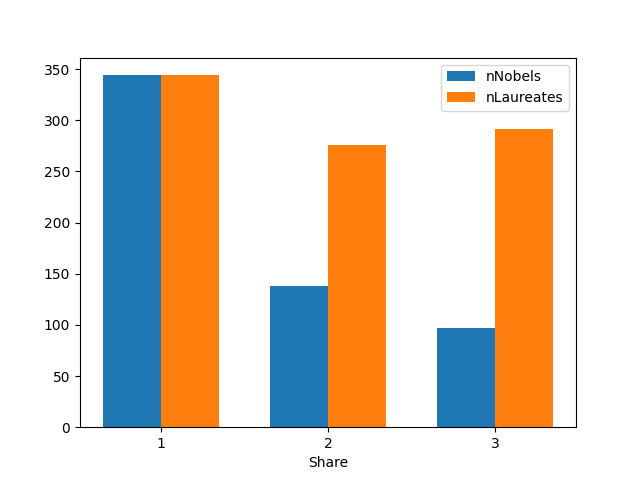
\includegraphics[width=0.7\linewidth]{../queries/plots/nobelShare.png}
	\caption{Distribution of Nobel Prizes among laureates}
	\label{fig:prizeShare}
\end{figure}

Another interesting fact is that the number of laureates who have won a Nobel Prize shared among three people (291)
is greater than the number of laureates who have won a Nobel Prize shared between two people (276).

\newpage

\section{Collaborations among Nobel laureates}

\begin{lstlisting}
PREFIX : <http://www.semanticweb.org/a3d/ontologies/2024/10/nobelOntology/>
PREFIX rdf: <http://www.w3.org/1999/02/22-rdf-syntax-ns#>
PREFIX foaf: <http://xmlns.com/foaf/0.1/>

SELECT ?title (GROUP_CONCAT(?name; SEPARATOR = ", ") AS ?laureates) WHERE {
    ?laureate rdf:type :Laureate .
    ?paper rdf:type :Paper ;
        :hasTitle ?title .
    ?laureate :hasWritten ?paper ;
        foaf:name ?name .
}
GROUP BY ?title
HAVING (COUNT(DISTINCT ?laureate) > 1)
\end{lstlisting}

\vspace{1em}

The goal of this query is to explore whether Nobel laureates collaborate with each other by co-authoring
scientific papers. As Table \ref{tab:laureates_collaboration} shows, among approximately 53,000 papers
and 904 laureates, only one paper was found to have been co-authored by multiple laureates.

\begin{table}[H]
	\caption{Paper co-authored by multiple Nobel Laureates}
	\centering
	\begin{tabular}{|l|l|}
		\hline
		\textbf{Title}                                             & \textbf{Laureates}                   \\ \hline
		Recursive Robust Estimation and Control Without Commitment & Lars Peter Hansen, Thomas J. Sargent \\ \hline
	\end{tabular}
	\label{tab:laureates_collaboration}
\end{table}

The two laureates won the Nobel Prize in 2013 and 2011, respectively, and the paper dates back to 2007.
Hence, these two laureates collaborate years before winning the Nobel Prize.

This result suggests that collaboration between Nobel laureates is extremely rare. However, it is important to
note that this outcome should not be taken as definitive, as the datasets used represent only a portion of all
existing papers and laureates. Nevertheless, it provides an interesting insight into the rarity of such
collaborations, offering a percentage-based perspective on how seldom laureates join forces to produce scientific
work.

\newpage

\section{Relationship between funding allocated for R\&D and possibility of winning a Nobel Prize}

\begin{lstlisting}
PREFIX : <http://www.semanticweb.org/a3d/ontologies/2024/10/nobelOntology/>
PREFIX rdf: <http://www.w3.org/1999/02/22-rdf-syntax-ns#>
PREFIX xsd: <http://www.w3.org/2001/XMLSchema#>

SELECT ?year ?topCountry (COUNT(?laureate) AS ?numLaureates) (COALESCE(CEIL(?fundingAmount), 0) as ?totalFunding) WHERE {
    {
        SELECT ?country WHERE {
            ?laureate rdf:type :Laureate ;
                      :worksFor ?organization .
            ?organization :basedIn ?city .
            ?city :locatedIn ?country .
        }
        GROUP BY ?country
        ORDER BY DESC(COUNT(DISTINCT ?laureate))
        LIMIT 3
    }
    BIND(?country AS ?topCountry)

    {
        SELECT DISTINCT ?year WHERE {
            ?nobelPrize :hasYear ?year .
            FILTER(?year < "2017"^^xsd:gYear)
        }
    }

    OPTIONAL {
        ?laureate rdf:type :Laureate ;
                  :hasWon ?nobelPrize ;
                  :worksFor ?organization .
        ?organization :basedIn ?city .
        ?nobelPrize :hasYear ?year .
        ?city :locatedIn ?topCountry .
    }

    OPTIONAL {
        ?topCountry :hasFunded ?funding .
        ?funding :hasYear ?year ;
                  :hasAmount ?fundingAmount .
    }
}
GROUP BY ?year ?topCountry ?fundingAmount
ORDER BY DESC(?year) ?topCountry
\end{lstlisting}

\vspace{1em}

With this query, we identified the top three countries with the highest number of Nobel laureates that were affiliated
to an organization there when they won the Nobel Prize, along with the annual amount of funding allocated to
research and development (R\&D) by these nations. To ensure data consistency, we limited our focus exclusively to
the years between 2000 and 2016.

\begin{figure}[H]
	\centering
	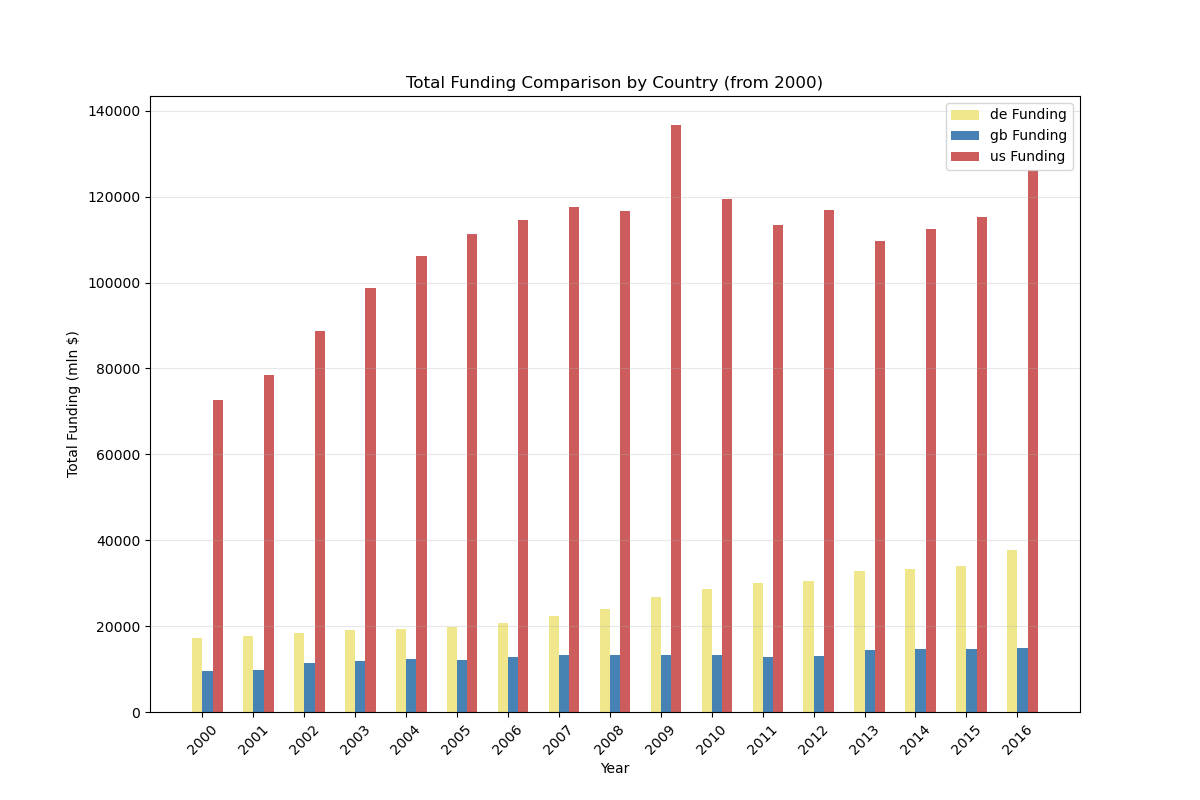
\includegraphics[width=0.8\textwidth]{../queries/plots/funding_comparison_by_country.png}
	\caption{Funding comparison by Country}
	\label{fig:fundings_per_country}
\end{figure}

\begin{figure}[H]
	\centering
	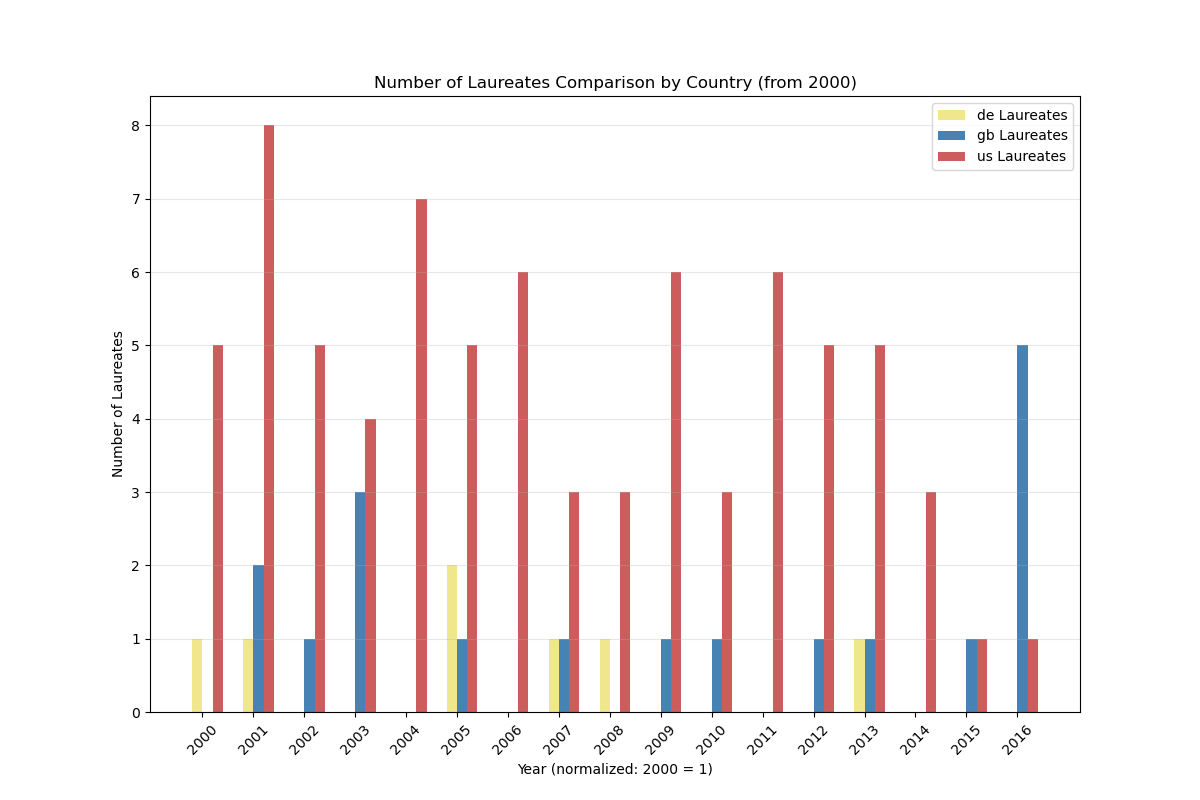
\includegraphics[width=0.8\textwidth]{../queries/plots/laureates_comparison_by_country.png}
	\caption{Laureates comparison by Country}
	\label{fig:laureates_per_country}
\end{figure}

The charts in Figures \ref{fig:fundings_per_country} and \ref{fig:laureates_per_country} at first seem to show
a correlation between R\&D funding and the number of Nobel laureates. This is especially true for the
United States, which dominates both metrics. The large investments in research seem to clearly support significant
achievements, resulting in more laureates each year. \\

However, when we look more closely, this trend does not apply everywhere. For example, Germany and Great Britain
show different patterns. The charts indicate that Germany's increasing R\&D funding over the years has not led
to more Nobel laureates. On the other hand, Great Britain, with lower and more stable funding levels, has
produced more laureates than Germany. This suggests that the link between funding and Nobel prizes is not always
straightforward. \\

In this case, the data and charts alone do not allow us to draw clear conclusions. While it is true that higher
funding supports development, Nobel-winning discoveries do not always follow trends reagarding money. With this,
we can conclude that this kind of discoveries generally come from exceptional minds and sparks of genius that
go beyond the usual patterns.

\newpage

\section{Laureates that won multiple Nobels}

\begin{lstlisting}
PREFIX : <http://www.semanticweb.org/a3d/ontologies/2024/10/nobelOntology/>
PREFIX xsd: <http://www.w3.org/2001/XMLSchema#>

SELECT ?laureate (COUNT(?nobel) AS ?numNobels) (GROUP_CONCAT(DISTINCT ?category; SEPARATOR = ", ") AS ?categories) WHERE {
    ?laureate :hasWon ?nobel .
    ?nobel :hasNobelCategory ?category .
}
GROUP BY ?laureate
HAVING (?numNobels > 1)
ORDER BY DESC (?numNobels)
\end{lstlisting}

\vspace{1em}

With this query we aim to discover laureates that won multiple Nobel Prizes and for which categories.\\
Table \ref{tab:moreThanOneNobel} highlights that only six laureates have been awarded multiple times and only three
Nobel categories have repeated winners.

\begin{table}[H]
	\centering
	\caption{Laureates who won more than one Nobel Prize}
	\begin{tabular}{|l|c|l|}
		\hline
		\textbf{Laureate}                      & \textbf{Number of Nobels won} & \textbf{Categories} \\ \hline
		Comite International De La Croix-Rouge & 3                             & Peace               \\ \hline
		Frederick Sanger                       & 2                             & Chemistry           \\ \hline
		John Bardeen                           & 2                             & Physics             \\ \hline
		Linus Carl Pauling                     & 2                             & Chemistry, Peace    \\ \hline
		Marie Curie                            & 2                             & Physics, Chemistry  \\ \hline
		UNHCR                                  & 2                             & Peace               \\ \hline
	\end{tabular}
	\label{tab:moreThanOneNobel}
\end{table}

It is interesting to note that all of these individuals or organizations won a prize in the same category,
or a similar one in the case of Marie Curie, except for one. Linus Carl Pauling won both the Chemistry and Peace Nobel Prizes,
suggesting that he was not only a scientist but also a socially engaged figure.\\
Additionally, no repeat winners are found in the categories of Economics, Literature and Medicine.
For Economics and Literature this absence might be partially attributed to the average high age of Nobel Prize
winners in these fields, as further analyzed in Section \ref{winners age}.\\

\newpage

\section{Number of papers published from the most important venues over the years}

\begin{lstlisting}
PREFIX : <http://www.semanticweb.org/a3d/ontologies/2024/10/nobelOntology/>

SELECT ?venue ?year (COUNT(?paper) AS ?numPapers) WHERE {
    # Get the most important venues (the ones with more than 800 papers published)
    {
        SELECT ?venue (COUNT(?paper) AS ?totPapers) WHERE {
            ?paper :publishedIn ?venue .
        }
        GROUP BY ?venue
        HAVING (?totPapers > 800)
        ORDER BY DESC (?totPapers)
    }

    # Get the number of paper published in the most important venues for each year
    ?paper :publishedIn ?venue ;
        :hasYear ?year .
}
GROUP BY ?venue ?year
ORDER BY ASC (?year)
\end{lstlisting}

\vspace{1em}

This query returns the number of papers published over the years by major
venues (those with more than 800 papers published, according to our dataset).

Figure \ref{fig:papersPerVenue} shows the trends of the six major research venues.

\begin{figure}[H]
	\centering
	\label{fig:papersPerVenue}
	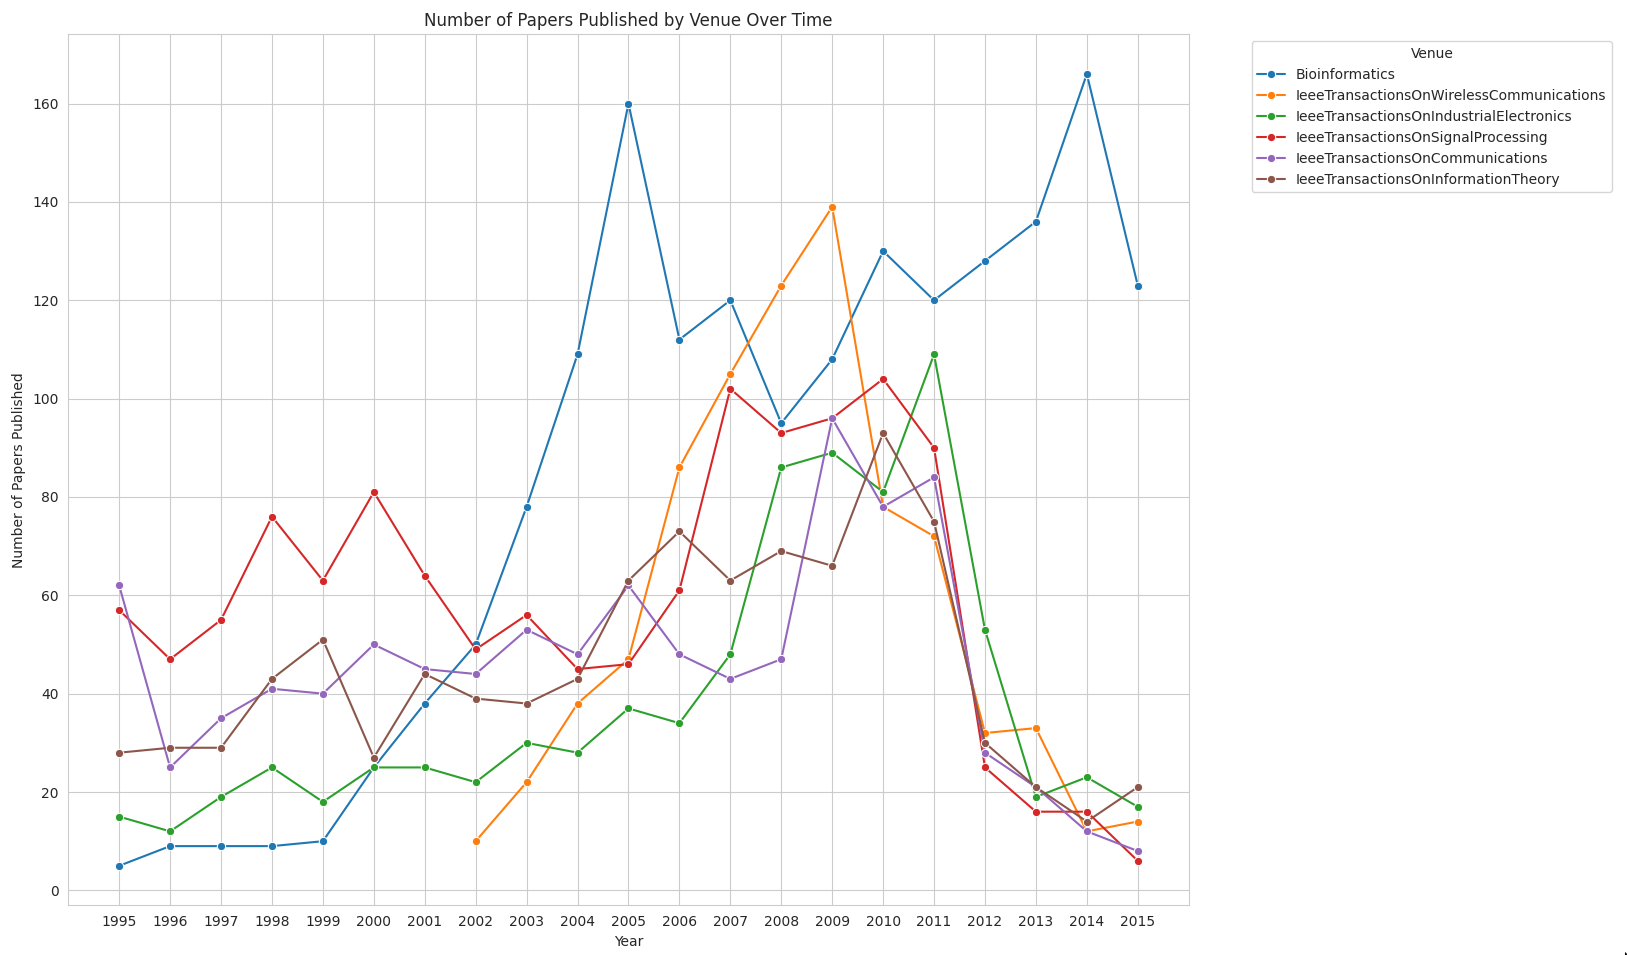
\includegraphics[width=\textwidth]{../queries/plots/papersPerVenue.png}
    \caption{Number of papers published by Venue per year}
\end{figure}

In recent years, Bioinformatics could be considered one of the most influential
venue because of its consistently higher number of papers published compared to others.
IEEE venues are the most prominent in the fields of information and tecnology.\\
For instance, in 2009 the research community focused more on the field of
communications.
That same year, the Physics Nobel Prize was awarded for "groundbreaking achievements
concerning the transmission of light in fibers for optical communication".

\newpage

\section{Number of papers published for each Nobel category}
\begin{lstlisting}
PREFIX skos: <http://www.w3.org/2004/02/skos/core#>
PREFIX : <http://www.semanticweb.org/a3d/ontologies/2024/10/nobelOntology/>

SELECT ?year ?category (SUM(?howmany) AS ?totalPapers) WHERE {
    {
        SELECT ?year ?category (COUNT(DISTINCT ?paper) AS ?howmany) WHERE {
            ?journal :hasJournalCategory ?category .
            :journalCategoryScheme skos:hasTopConcept ?category .
            ?paper :publishedIn ?journal ;
                :hasYear ?year .
        }
        GROUP BY ?year ?category
    }
    UNION
    {
        SELECT ?year ?category (COUNT(DISTINCT ?paper) AS ?howmany) WHERE {
            ?journal :hasJournalCategory ?cat .
            ?cat skos:broaderTransitive ?category .
            ?paper :publishedIn ?journal ;
                :hasYear ?year .
        }
        GROUP BY ?year ?category
    }
}
GROUP BY ?year ?category
ORDER BY DESC (?totalPapers)
\end{lstlisting}

\vspace{1em}

This query allows us to extract, for each year, the number of scientific articles published for each Nobel Prize category. This approach offers a comprehensive view
of the distribution of published papers over time, allowing us to identify which research areas, related to Nobel categories, have attracted the most attention
from scholars over the time.\\

As we can see from Figure \ref{fig:papersPerCategory}, in recent years the most studied field is Medicine which attracted more and more attention since 2002, while in the
90s the most studied one was Economics, which reached its peak in 2008, probably due to the economic crisis of that time.

\begin{figure}[ht]
	\label{fig:papersPerCategory}
	\centering
	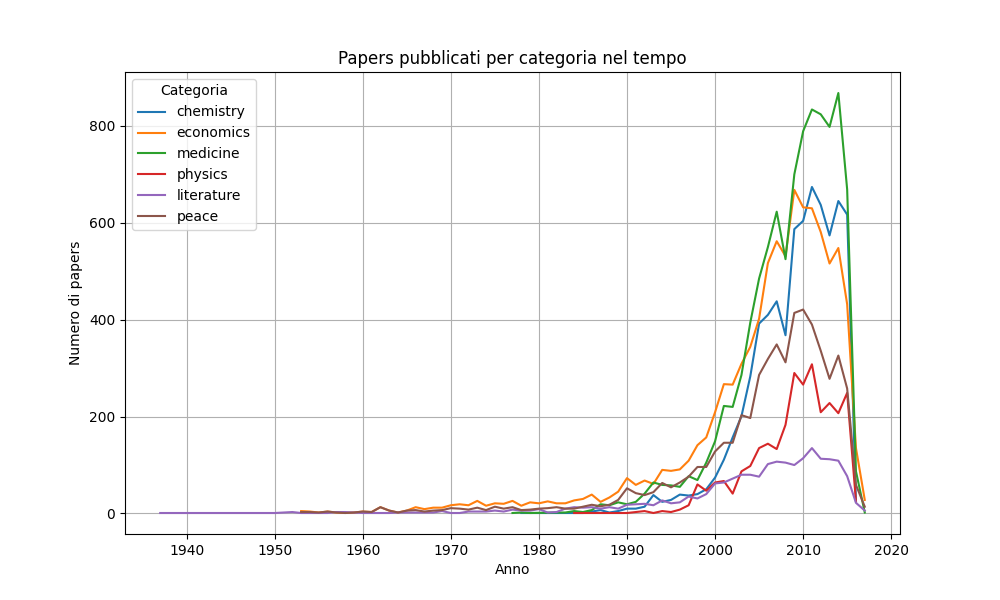
\includegraphics[width=0.9\textwidth]{../queries/plots/papersPerCategory.png}
    \caption{Published papers over the years per Category}
\end{figure}

\newpage

\section{Age analysis of Nobel Prize winners} \label{winners age}
\begin{lstlisting}
PREFIX : <http://www.semanticweb.org/a3d/ontologies/2024/10/nobelOntology/>
PREFIX foaf: <http://xmlns.com/foaf/0.1/>

SELECT ?category (MIN(?age) AS ?minAge) (ROUND(AVG(?age)) AS ?avgAge) (MAX(?age) AS ?maxAge) WHERE {
    ?laureate a :Laureate ;
        :birthDate ?birthDate ;
        :hasWon ?prize .
    ?prize :hasYear ?prizeYear ;
        :hasNobelCategory ?category .
    BIND (YEAR(?prizeYear) - YEAR(?birthDate) AS ?age)
}
GROUP BY ?category
\end{lstlisting}

\vspace{1em}

The data extracted from the query provides insights into the age at which individuals achieve great results in
their fields:

\begin{table}[H]
	\centering
	\caption{Age statistics of Nobel Prize winners by category}
	\begin{tabular}{|l|c|c|c|}
		\hline
		\textbf{Category} & \textbf{Min Age} & \textbf{Avg Age} & \textbf{Max Age} \\ \hline
		Chemistry         & 35               & 58               & 85               \\ \hline
		Economics         & 51               & 67               & 90               \\ \hline
		Literature        & 42               & 65               & 88               \\ \hline
		Medicine          & 32               & 58               & 87               \\ \hline
		Peace             & 17               & 61               & 87               \\ \hline
		Physics           & 25               & 55               & 88               \\ \hline
	\end{tabular}
	\label{tab:age_analysis}
\end{table}

Table \ref{tab:age_analysis} highlights notable trends in the ages of Nobel Prize winners:

\begin{itemize}
	\item \textbf{Economics}: With an average age of 67, this category has the highest average age.
	      This observation likely reflects the time required to develop groundbreaking theories and gain significant recognition in this field. Also the minimum age of 51 suggests that Nobel laureates in Economics often
	      achieve their recognition later in life.

	\item \textbf{Peace}: This category includes the youngest laureate, at only 17 years old.
	      The diversity in ages within this category (average age 61, maximum 87) reflects the variety of
	      contributions recognized, from lifelong efforts in diplomacy to impactful single events, such as activism
	      or humanitarian work.

	\item \textbf{Chemistry, Medicine, and Physics}: These science-related categories show similar average ages
	      (55-58 years) and a range of minimum ages (from 25 to 35 years). The relatively young ages of some laureates
	      in Physics (25) and Medicine (32) suggest that groundbreaking discoveries in these fields are sometimes made
	      early in a researcher's career, possibly during postdoctoral experiences.

	\item \textbf{Literature}: With an average age of 65, second only to Economics, and a minimum age of 42, this
	      category highlights the time often required for authors to improve and craft a masterpiece.
	      Furthermore, the Nobel Prize in Literature is frequently awarded in recognition of an author's
	      entire career, considering their overall contribution to the field rather than a single achievement.
\end{itemize}

\newpage

By digging deeper into the age data, we can perform an additional query to identify the youngest and oldest
Nobel Prize winners.

\begin{lstlisting}
PREFIX : <http://www.semanticweb.org/a3d/ontologies/2024/10/nobelOntology/>
PREFIX foaf: <http://xmlns.com/foaf/0.1/>

SELECT ?name ?birthDate ?prize ?age WHERE {
    {
        SELECT (MIN(YEAR(?prizeYear) - YEAR(?birthDate)) AS ?minAge) (MAX(YEAR(?prizeYear) - YEAR(?birthDate)) AS ?maxAge) WHERE {
            ?laureate a :Laureate ;
                foaf:name ?name ;
                :birthDate ?birthDate ;
                :hasWon ?prize .
            ?prize :hasYear ?prizeYear .
        }
    }

    ?laureate a :Laureate ;
        foaf:name ?name ;
        :birthDate ?birthDate ;
        :hasWon ?prize .
    ?prize :hasYear ?prizeYear .

    BIND (YEAR(?prizeYear) - YEAR(?birthDate) AS ?age)
    FILTER (?age = ?minAge || ?age = ?maxAge)
}
\end{lstlisting}

\vspace{1em}

The results are presented in Table \ref{tab:youngest_oldest}:

\begin{table}[H]
	\centering
	\caption{Youngest and oldest Nobel Prize winners}
	\begin{tabular}{|l|l|l|l|c|}
		\hline
		\textbf{Name}    & \textbf{Birth Date} & \textbf{Prize} & \textbf{Age} \\ \hline
		Leonid Hurwicz   & 1917-08-21          & Economics 2007 & 90           \\ \hline
		Malala Yousafzai & 1997-07-12          & Peace 2014     & 17           \\ \hline
	\end{tabular}
	\label{tab:youngest_oldest}
\end{table}

The youngest Nobel Prize winner is Malala Yousafzai, who received the Peace Prize in 2014 at the age of just 17.
Her recognition came as a result of her activism for girls' education and human rights, which gained international
attention and inspired millions worldwide.\\
The oldest Nobel laureate is Leonid Hurwicz, who was awarded the Nobel Prize in Economics in 2007 at the age of 90.
This result demonstrates a lifetime of work in economics, highlighting how breakthroughs in theoretical fields
often come from years and years of effort and experience.

\newpage

\section{Nobel laureates: birthplace vs. research location by state}
\begin{lstlisting}
PREFIX : <http://www.semanticweb.org/a3d/ontologies/2024/10/nobelOntology/>
PREFIX foaf: <http://xmlns.com/foaf/0.1/>

SELECT ?state ?bornIn ?bornAndWorkIn WHERE {
    {
        SELECT ?state (COUNT(DISTINCT ?laureate) AS ?bornIn) WHERE {
            ?laureate a :Laureate ;
                :bornIn ?city .
            ?city :locatedIn ?country .
            ?country foaf:name ?state .
        }
        GROUP BY ?state
    }
    {
        SELECT ?state (COUNT(distinct ?laureate) AS ?bornAndWorkIn) WHERE {
            ?laureate a :Laureate ;
                :worksFor ?organization ;
                :bornIn ?birthCity .
            ?organization :basedIn ?orgCity .
            ?orgCity :locatedIn ?country .
            ?birthCity :locatedIn ?country .
            ?country foaf:name ?state
        }
        GROUP BY ?state
    }
}
ORDER BY DESC (?bornIn)
\end{lstlisting}

\vspace{1em}

This query returns, for each state, the number of laureates who were born in that state but conducted research abroad, and the number of
laureates who were born in that state and conducted research there.\\
This allows us to understand how many Nobel Prize winners conducted research in their home country or abroad in order to earn the recognition.

Figure \ref{fig:laureatesComparison} displays the data returned by the query, while Table \ref{tab:laureates_active} reports the five states with the lowest percentage
of laureates active in research in their home country.\\
As expected, the US is the state with the highest number of laureates and also with the highest percentage
of active laureates in their home country (88\%), thanks to the large fundings allocated in R\&D, as seen before.\\
An interesting fact is that Japan, despite being the 7th country in terms of Nobel Prizes won, manages to retain nearly 67\% of its laureates
within its borders. On the other hand, Russia, despite being the 6th country in terms of Nobel Prizes won, has a retention rate of only 35\%.

\begin{table}[h!]
	\centering
	\caption{Laureates active in research in their home country}
	\begin{tabular}{|c|c|c|c|c|}
		\hline
		\textbf{State} & \textbf{Laureates} & \textbf{Laureates active in their home country} & \textbf{Percentage} \\ \hline
		Canada         & 19                 & 2                                               & 10,5\%              \\ \hline
		China          & 11                 & 2                                               & 18,2\%              \\ \hline
		Italy          & 19                 & 4                                               & 21\%                \\ \hline
		Austria        & 17                 & 4                                               & 23,5\%              \\ \hline
		Australia      & 11                 & 3                                               & 27,3\%              \\ \hline
	\end{tabular}
	\label{tab:laureates_active}
\end{table}

\begin{figure}[H]
	\centering
	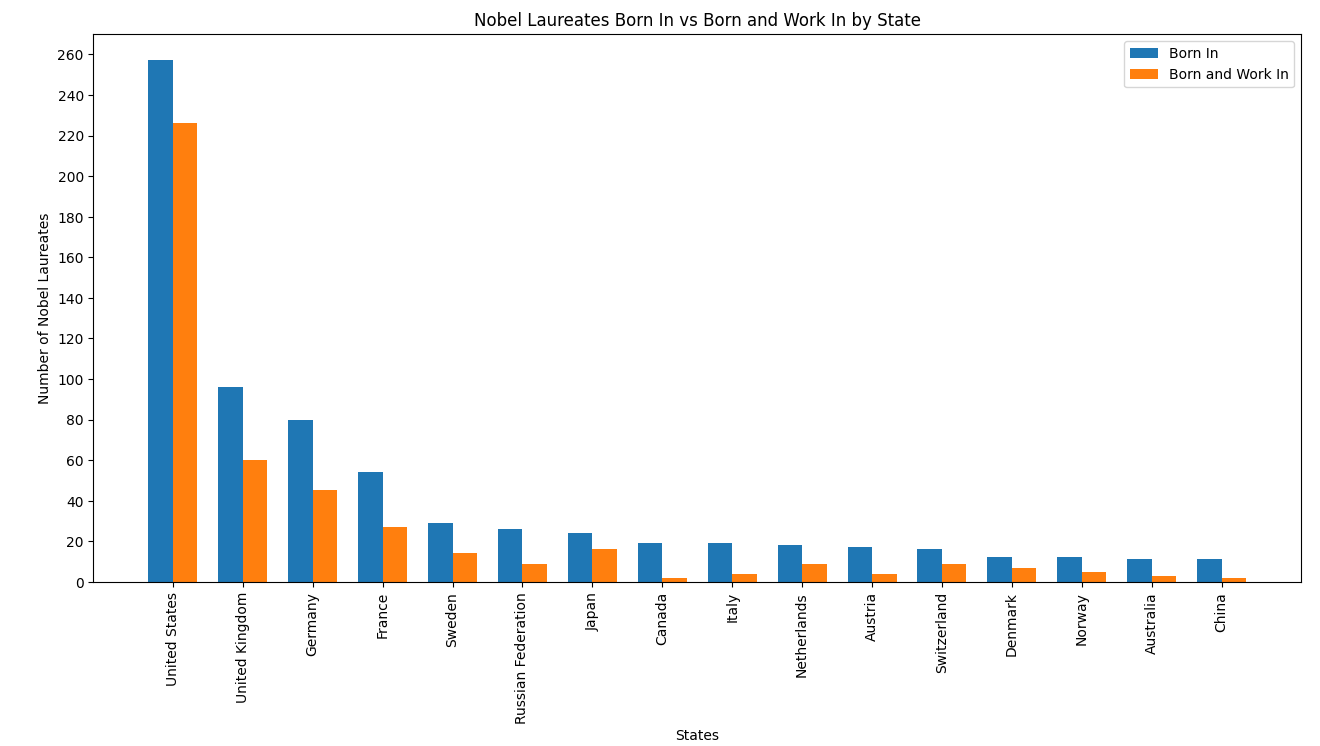
\includegraphics[width=\textwidth]{../queries/plots/laureatesComparison.png}
	\caption{The plot shows for each state two columns. The blue one indicates the number of laureates born in that state but active abroad.
		The orange one indicates the number of laureates born and active in that state}
	\label{fig:laureatesComparison}
\end{figure}

\end{document}
